\chapter{Introduction}
\label{ch:introduction}

Cancer is a widespread and often lethal disease\cite{10.1001/jamaoncol.2021.6987} where body cells mutate in a way that increases their cell division speed as well as their lifetime, while also evading immune responses. There are many possible treatment methods like surgery, chemotherapy, or radiation therapy, but their effectiveness often depends on the exact type of tumor. Tumors however are heterogenous: Individual tumor cells may mutate again and form new subclones that compete against others \cite{nik2012life}. Treating the dominant subclones however seems to provide an advantage for previously minor, resistant subclones \cite{gillies2012evolutionary}. Therefore, knowledge of existing subclones and their evolutionary history may help future treatments \cite{greaves2012clonal, stratton2009cancer, swanton2012intratumor}.

Bulk sequencing of tumor cells and analysing the found mutations appears to be already widely used, but seems to miss smaller, upcoming variants that are averaged out in the mass of cells \cite{navin2014cancer}. Therefore, research has been done to utilise single cell sequencing. With this technique, the exact genome of individual cells can be identified and compared against other cells. However, it also comes with high error rates and parts of a cell's genome are often lost during the process \cite{tree2016}. It is therefore very hard to identify which subclones actually exist and how they are related. There is therefore a need for algorithms that compute the most-likely mutation history. Such an algorithm is \acs{SCITE}\acused{SCITE} \cite{tree2016}, which is short for \acl{SCITE}.

\acp{FPGA} are computer chips that contain a lattice of logic, computation, and memory units that are connected via programmable connections. They can be used like complete, reprogrammable computer chips and have already been used extensively for chip prototyping and verification \cite{rodriguez2007features}. In recent years they have also become interesting as computation accelerators for \ac{HPC} users due to their low power consumption compared to their performance \cite{betkaoui2010comparing}. However, developing efficient \ac{FPGA} designs is often tedious since compiling them may take multiple hours and naive designs are often multiple orders of magnitudes worse than optimized ones \cite{betkaoui2010comparing}.

The original authors of \ac{SCITE} provided a functional, but rather unoptimized implementation of their algorithm. There is however an unpublished report by Dominik Ernst et al. \cite{ernst2020Performance} about their efforts to optimize the algorithm for parallel CPU architectures. Their list of parallelizable subtasks also contained entries that can be exploited well on \acp{FPGA}. Our general goal for this thesis is therefore to exploit these opportunities and develop an efficient implementation of \ac{SCITE} for \acp{FPGA}. 

\section{Background}

\ac{SCITE} is designed for the following scenario: A physician has been able to extract tumor tissue from a patient, either through surgery or other methods. Then, individual cells are extracted from the tissue, their genome is sequenced, and the resulting sequence of base pairs is scanned for subsequences, so-called genes. These genes may either be present in their most common form or in a less common, mutated way. The scanner identifies these mutations and produces a mutation matrix with an entry for every cell-gene-combination, where a 1 denotes that the cell has this mutation and 0 denotes the opposite.

This matrix itself may already be interesting to evaluate, but it should be handled with caution since the process of amplifying and sequencing the genome is very prone to errors. While there is often only a small chance to identify a mutation where there isn't one (false positives), there is a high change to miss a mutation (false negative). Lastly, there is also a high chance that genes are simply lost in the process. In this case, the matrix contains a third ``unknown'' entry encoded as a 2.

\todo[inline]{Research probabilites in the real world}

It is however possible to catch some of these errors with some assumptions on how mutations are introduced to the tumor: First of all, we assume that there are no mutations in the observed genes outside of the tumor. This means that before the tumor came into existence, there were only perfectly normal cells. When a cell replicates itself, it creates a perfect copy of its own genome for one of the two new cells, and these two cells pass their genome to their subclones too. However, cells can not share or swap their genome. If a gene of a cell's genome mutates, the altered genome will therefore be passed down to its subclones and its subclones only. If we then also assume that every gene only mutates once in the whole history of the tumor (the so-called infinite sites assumption), we can arrange the mutations in their order of occurrence.

\begin{figure}
    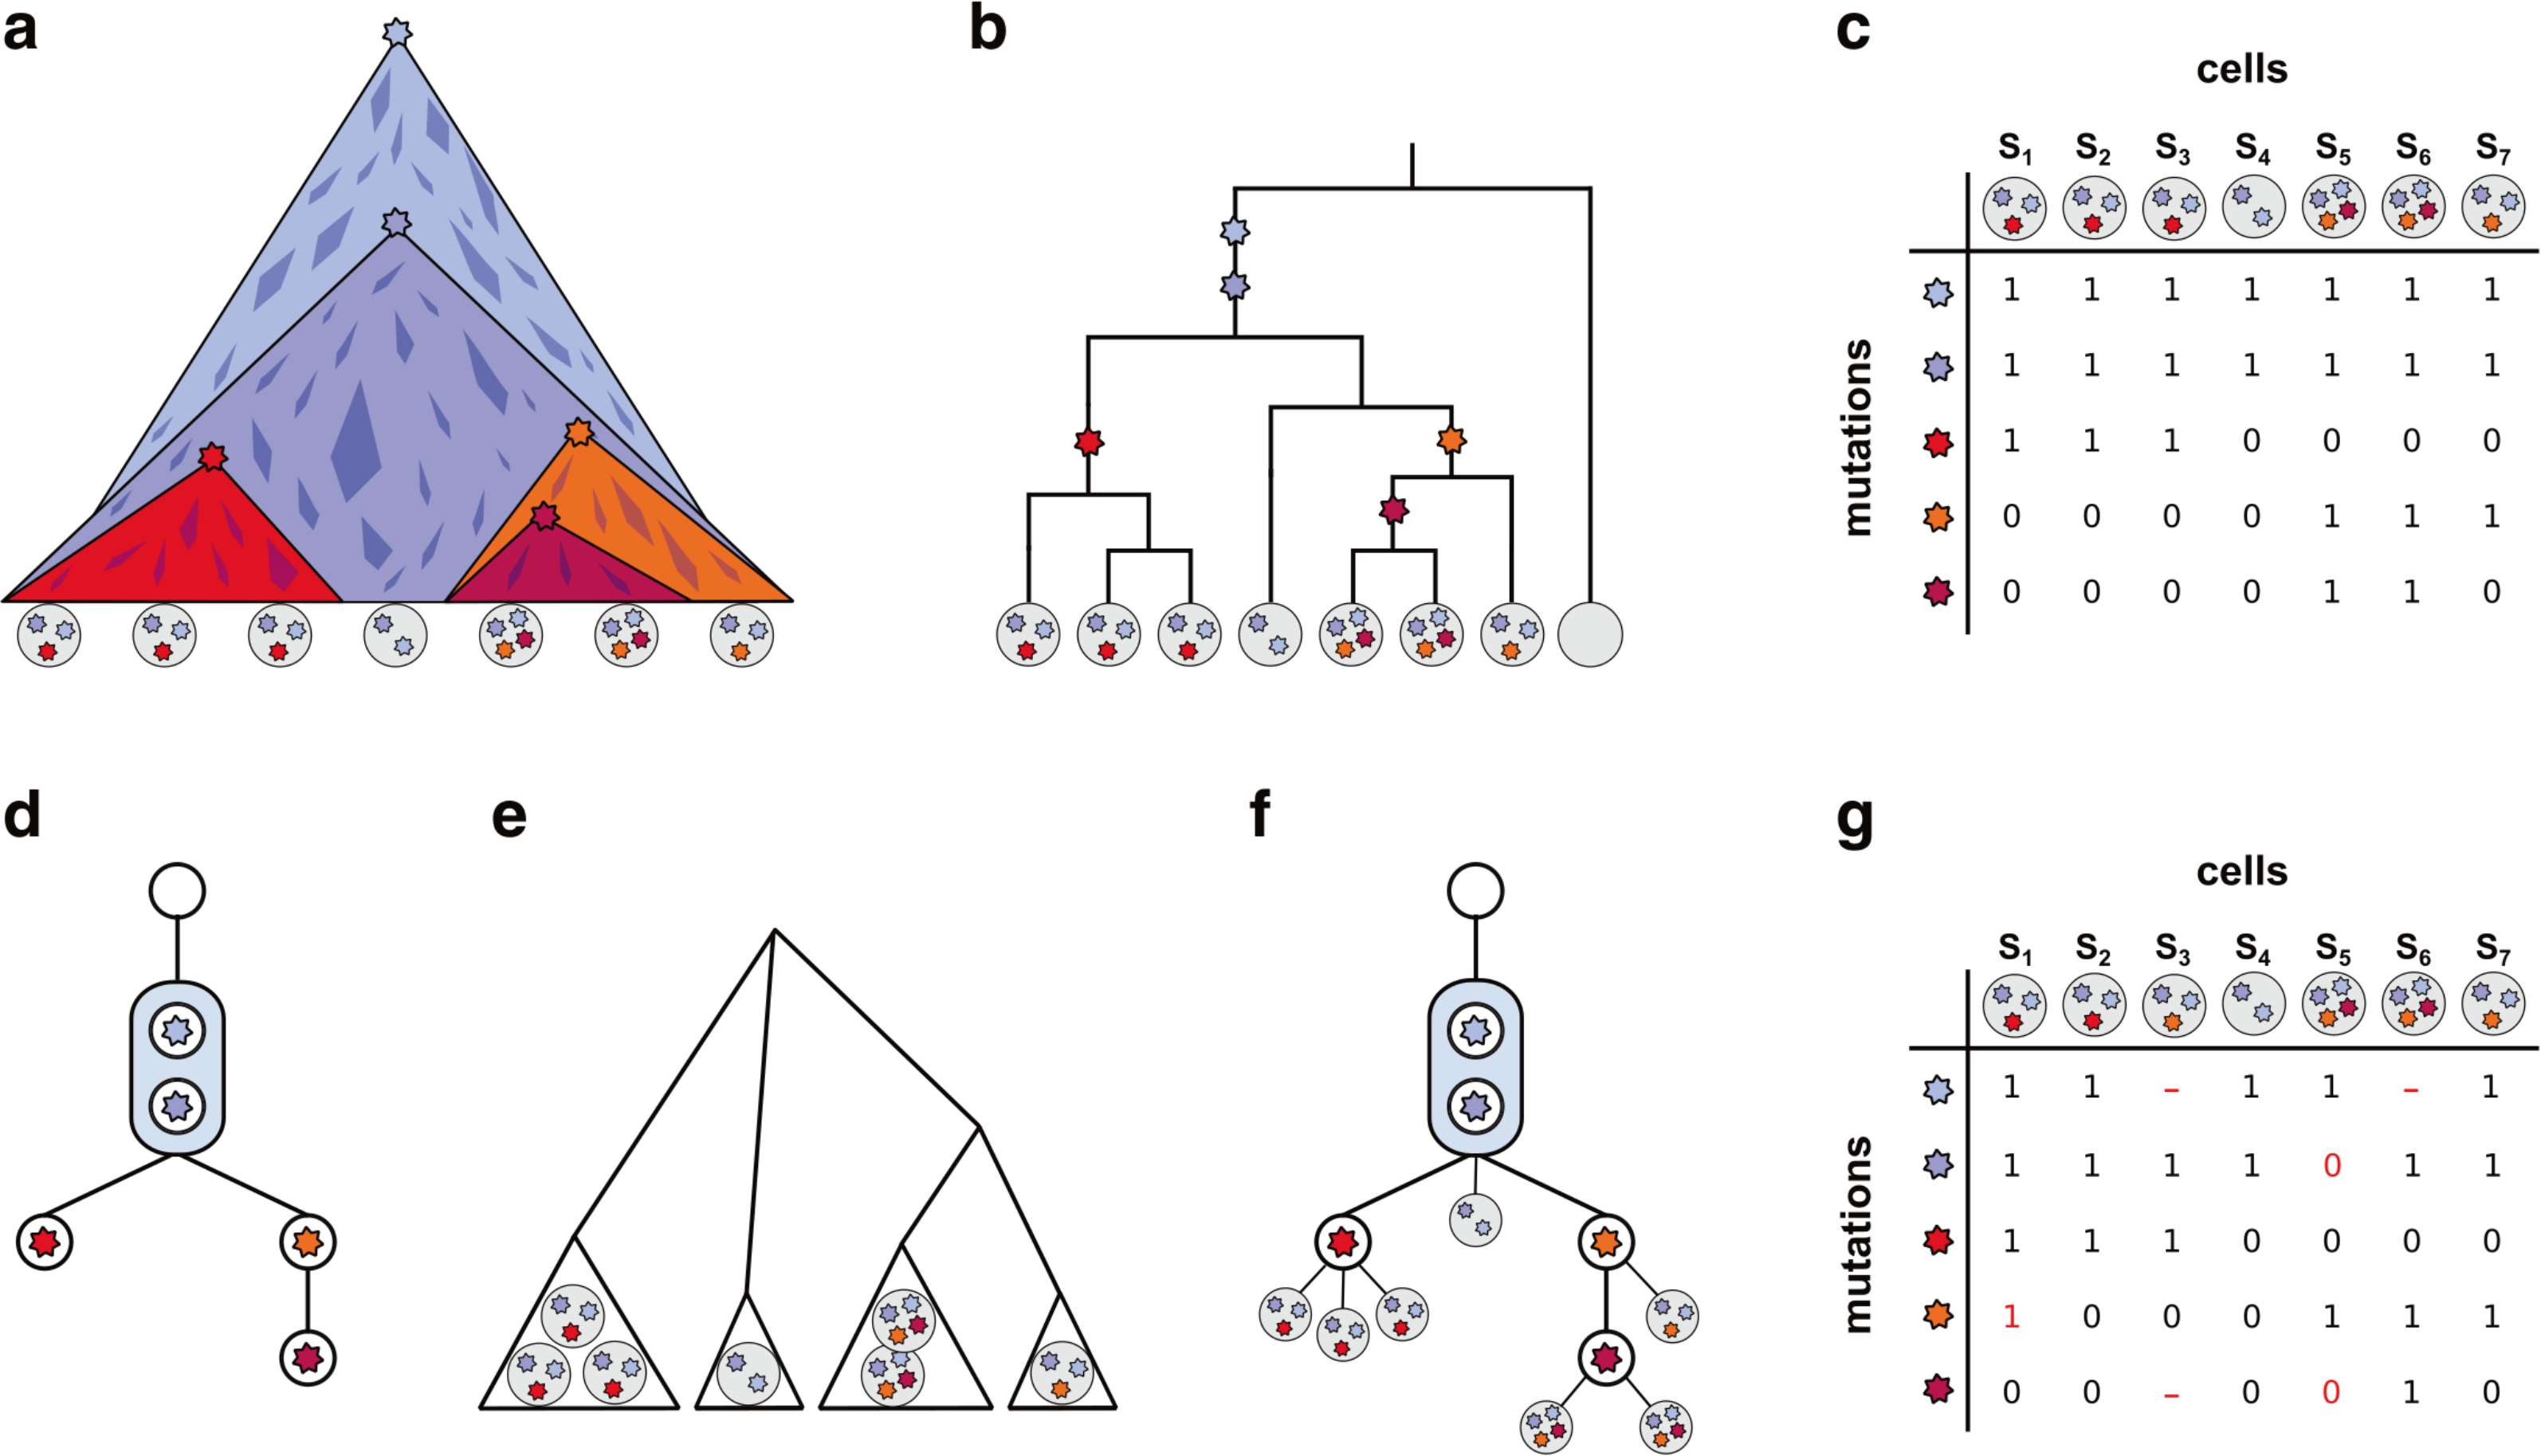
\includegraphics[width=\textwidth]{figures/example_tree.png}
    \centering
    \label{fig:example_tree}
    \caption{``Tumor evolution and cell phylogeny. \textbf{a} Schematic representation of tumor evolution with time progressing downwards. Stars denote new mutations leading to subclone expansion. The quadrangles belong to minor extinct subclones with no traces in the present-day populations. The mutations founding these clones may not have induced a sufficient growth advantage to have surviving descendant cells or may have been lost by chance. The gray discs on the bottom denote single cells sequenced after tumor removal. The stars they contain indicate the mutations observed in the cell. \textbf{b} Binary genealogical tree of the sequenced cells. An empty disc represents a normal somatic cell, which is an outgroup for the tumor cells. \textbf{c} Binary mutation matrix representing the mutation status of the sequenced tumor cells. A zero entry denotes the absence of a mutation in the respective cell, while a one denotes its presence. \textbf{d} The perfect phylogeny represented as a mutation tree, the partial (temporal) order of the mutation events. Mutations are summarized in a single node when their order is unidentifiable from the sampled cells, as is the case here for the two top-most mutations with the matrix from (c). \textbf{e} Hierarchical subclone structure. Cells with identical mutation profiles cluster into subclones, which serve as taxa in this phylogenetic tree. \textbf{f} Mutation tree with single-cell samples attached. \textbf{g} Noisy mutation matrix with missing values. The red numbers indicate flipped mutation states with respect to the true mutation matrix in (c). For 0→ 1, a false positive, the mutation is called but not present in the cell. For 1→ 0, a false negative, the mutation is not called but present in the cell, most likely due to allelic dropout during the DNA amplification. The red dash indicates a missing value; it is unknown whether the site is mutated or in the normal state in this cell.'' Copyright (C) Katharina Jahn et al., CC-BY 4.0, screenshot and cropped}
\end{figure}

\todo[inline]{Describe example tree, cell attachment, assumed true mutation matrix, concept of likelihood}

Finding a maximum-likelihood tree however is not easy. If $n$ genes are considered, the number of trees is in $O(n!)$ (Prüfer Codes), which makes an exhaustive search impractical. Jahn et al. therefore designed \ac{SCITE} as a \ac{MCMC} algorithm to empirically find the maximum likelihood tree.

\todo[inline]{Find a good paper for Prüfercodes}

A Monte Carlo algorithm runs a random experiment that produces a possible solution to a problem and evaluates how well the generated solution solves the problem. This loop of generating and evaluating a solution is then repeated multiple times and the result is the best solution the algorithm has encountered. In theory, it would suffice if the experiment had a probability greater than zero to produce a good solution, but in order to improve the solution quality and to reduce the required repetitions, one would use an experiment that produces the best solutions with a higher probability than worse solutions and that can be repeated quickly. As the name implies, \ac{MCMC} algorithms are Monte Carlo algorithms that simulate a Markov Chain to produce solutions. The advantage of using Markov Chains is that the next sample may depend on the previous one and the algorithm therefore only needs to introduce small changes to the solution. This is often faster than generating a new solution from scratch and if the current sample is already a good solution, the change may preserve some of its quality. However, a designer of a \ac{MCMC} algorithm has to make sure that the chain actually converges on the desired distribution.

\section{Goals of the Thesis}

\todo[inline]{Rewrite this section to present tense, shorten it.}

With the algorithm introduced and possible performance problems identified, we can formulate our goals: We plan to implement \ac{SCITE} for the Intel Stratix 10 GX 2800 \acp{FPGA} of the Noctua supercomputers at the Paderborn University using the Intel oneAPI/DPC++/SYCL toolchain, since we have the most experience with this target and toolchain. We want to maximize the number of markov chain steps executed per second, what we call henceforth call throughput, while still producing results of similar likelihood to the original reference implementation. We want to achieve at least as much throughput as the original reference implementation and if possible, we also want to achieve more throughput than the implementation of Ernst et al. \cite{ernst2020Performance}. This is however an optional goal since there is a possibility that we encounter optimization problems that can not be resolved in time and since we do not have access to the implementation or its performance figures yet. We also want to develop benchmarking and result validation tools for our implementation. This requires a performance model that can accurately predict and explain the runtime of the design given the input dimensions and performance parameters, as well as a hypothesis test framework to check whether our implementation's quality matches those of the reference implementation. Lastly, we also want to try to identify the changes required to adapt our implementation to \ac{infSCITE} and to evaluate whether it is feasible. However, this is also an optional goal since it is not essential to our main goal of performance engineering. Figure \ref{fig:goals} contains a summarized list of goals.

\begin{figure}
    \begin{itemize}
        \item Implement \ac{SCITE} for \acp{FPGA}
        \begin{itemize}
            \item Maximize throughput (number of markov chain steps executed per second)
            \item Produce solutions of similar likelihood as the original reference implementation
            \item Achieve at least as much throughput as the original reference implementation
            \item (Optional) Achieve more throughput than the implementation by Ernst et al. \cite{ernst2020Performance}.
        \end{itemize}
        \item Develop benchmarking and validation tools
        \begin{itemize}
            \item Develop a performance model for runtime prediction and explanation
            \item Develop a hypothesis test framework for the result quality
        \end{itemize}
        \item (Optional) Identify and evaluate changes required for \ac{infSCITE} adaptation
    \end{itemize}

    \centering
    \caption{Summary/Overview of the goals of the thesis}
    \label{fig:goals}
\end{figure}

In order to fullfil these goals, we will start with an initial implementation of the algorithm. This implementation may be naive and therefore possibly inefficient, but it should be functional and correct. Parallel to that, we will start to set up the verification and benchmarking system to establish the baseline of the initial FPGA implementation and the reference implementation. Once the foundations are established, we can begin to optimize. There is not much sense in planning this task since it heavily depends on the bottlenecks at hand, but it will probably result in repeated iterations of profiling, identification of bottlenecks, research in existing solutions, implementing existing or original ideas and analyzing the changes. We will write-up the findings from all analysis stages, which will aid use in the last phase: Writing the thesis and proofreading it. There, we will describe what performance we could achieve, which bottlenecks we have encountered, how we have resolved them, and how our decisions have affected the adaptability to \ac{infSCITE}. More precisely, we plan to use the structure in Figure \ref{fig:thesisstructure} for the thesis.

\begin{figure}
    \begin{itemize}
        \item Introduction
        \begin{itemize}
            \item Motivation
            \item Background
            \item Related Work
        \end{itemize}
        \item Implementation
        \begin{itemize}
            \item Notable Bottlenecks and Solutions
            \item Adaptability of \ac{infSCITE}
            \item Verification \& Benchmarking Framework
        \end{itemize}
        \item Results
        \begin{itemize}
            \item Result likelihood
            \item Performance
        \end{itemize}
        \item Conclusion
    \end{itemize}
    \centering
    \caption{Planned structure of thesis}
    \label{fig:thesisstructure}
\end{figure}

\begin{figure}
    % Modified from https://git.cs.uni-paderborn.de/syssec/templates/exposee
    \begin{ganttchart}
        [x unit=0.5cm, %extend sheets to 1cm
        ]{1}{18}
        \gantttitle[title label node/.append style={below left=7pt and -3pt}]{WEEKS:\quad1}{1}
        \gantttitlelist{2,...,18}{1} \\
        \ganttgroup{Initial Implementation}{1}{4} \\
        \ganttgroup{Verification \& Benchmarking}{2}{6} \\
        \ganttgroup{Optimization}{5}{12} \\
        \ganttgroup{Writing \& Proofreading}{13}{18}
    \end{ganttchart}
    \centering
    \caption{Worst-Case work schedule}
    \label{fig:worstschedule}
\end{figure}

According to the regulations, the workload of the thesis is supposed to contain nine weeks of full time labor, which is equivalent to 18 weeks of half time labor. The deadline for handing the thesis in is five months, which is approximately equivalent to 21 to 22 weeks and leaves a buffer of three to four weeks. We assume that the initial implementation will take approximately four weeks, as we will need to rewrite the complete application due to its heavy use of dynamic memory in datastructures and the kernel code, as well as its imperative structure. Benchmarking will be rather easy with our experience in profiling oneAPI FPGA designs, but since we have no experience in statistical verification, we can not actually make a good prediction for the required time. For writing the thesis, other students have quoted approximately four to six weeks of half-time work for thesis writing and proofreading, which leaves approximately nine to thirteen weeks between the initial implementation and writing the thesis for optimization. The resulting worst-case work schedule is visualized in Figure \ref{fig:worstschedule}.
